\chapter{Cameras}



\section{Synchronization (PPT+PPS)}
Fast mode \approx $50\mu s$. Accurate mode prohibits $20hz$ refresh rate.
Verified using oscilloscope and analog output.
Cameras report ptp offset, but without a proper oscilloscope it is hard to verify if this is correct.


\section{Real time image processing}
Asyncio, subprocessing, queues and a lot of pain.



\section{Calibration}


\section{Network management}

Using network card.
A lot of configuration has to be done -> Python script.
\subsection*{Network card}
\subsection*{Jumbo Frames}
\subsection*{Receive Buffers}
\subsection*{Ip Address Assignment}
Local network for each eth device.
Assure no overlap.
\subsection*{Reverse Path Filtering}



\section{Compression}
H265 for video, JPEG for images.
\subsection*{gstreamer}
\subsection*{Hardware acceleration}
Verified with \gls{jtop}.

\section{Custom debayering (GPU?)}
Not needed for now, but could be useful for future work.
Currently using OpenCV debayering.

An idea is to combine debayering, I420 conversion and polarization representations into one kernel.

\section{Polarization stuff}
Save all 4 polarization channels.
Gives more options for postprocessing in cases of ie saturation.

\section{Testing and verification of the system?}
Check compression loss.

\subsubsection{Receive Buffers}
\begin{figure}
    \centering
    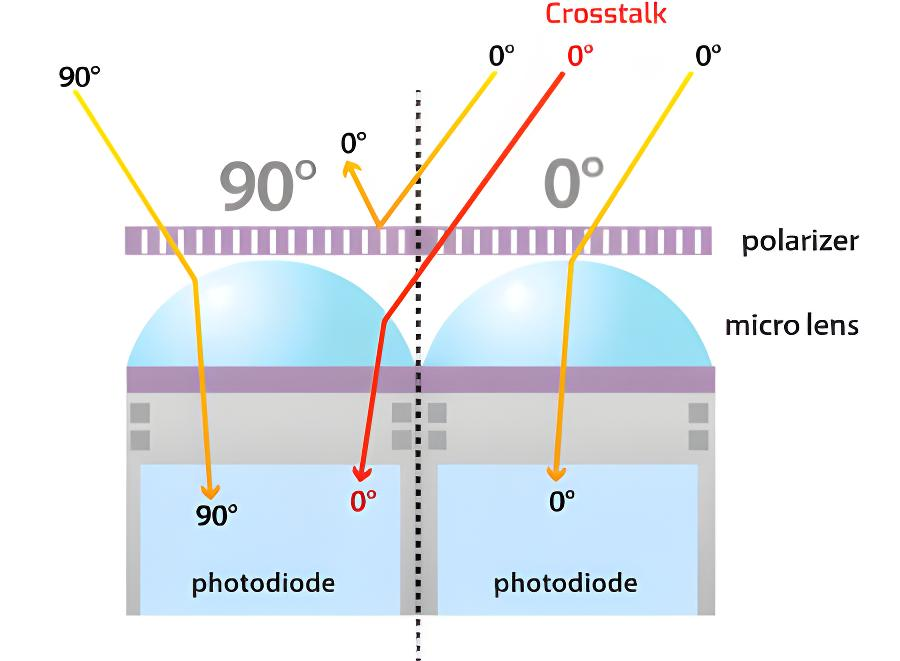
\includegraphics[width=0.8\textwidth]{figures/crosstalk_upscaled.jpg}
    \caption{$0^{\circ}$ polarized light is entering the pixel meant to detect $90^{\circ}$ and will be incorrectly detected as $90^{\circ}$.  This crosstalk error happens because the polarization array is placed above the micro lens \cite{lucidvisionlabsPolarizationExplainedSony2018}}
    \label{fig:camera_crosstalk}
\end{figure}
% \end{figure}
\begin{figure}
    \centering
    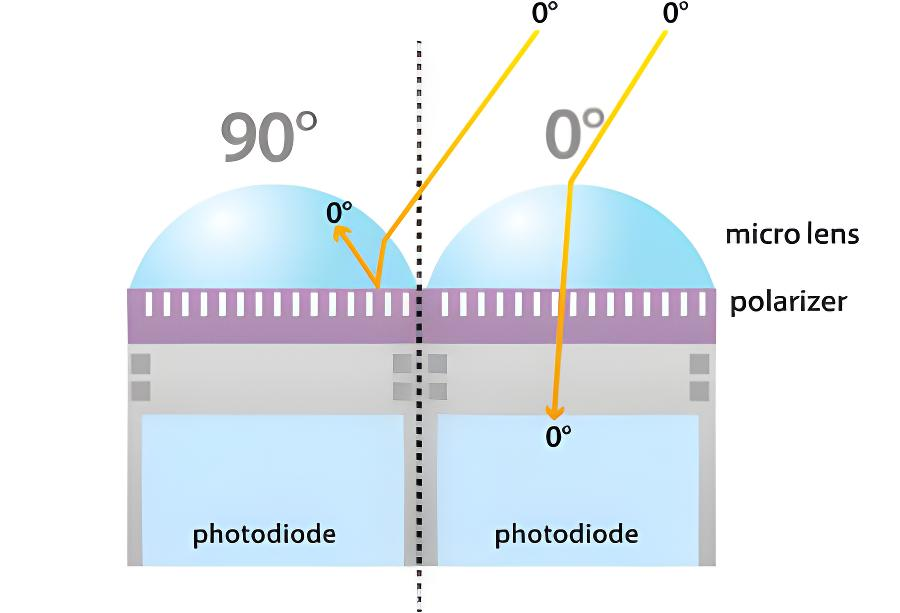
\includegraphics[width=0.8\textwidth]{figures/crosstalk_off_upscaled.jpg}
    \caption{Sony's polarization sensor reduces the chance of crosstalk thanks to the polarizer array being placed on-chip. The $0^{\circ}$ polarized light is unable to enter the pixel meant to detect only $90^{\circ}$ \cite{lucidvisionlabsPolarizationExplainedSony2018}}
    \label{fig:camera_no_crosstalk}
\end{figure}
